\section{Spotřeba}
Podstatným parametrem zařízení je~jeho spotřeba a~tedy doba, po~kterou může běžet z~powerbanky.

V~rámci prostého měření vstupního proudu při využívání všech periferií vyjma WiFi a Bluetooth, jsem při napětí \(5~V\) změřil vstupní proud v~rozsahu \(35~mA\) až~\(195~mA\) v~závislosti na~aktuálním využití LED kruhu.
Provozní příkon je~tedy v~rozsahu \(35 [mA] \cdot 5~[V] = 175 [mW]\) až~\(195 [mA] \cdot 5~[V] = 975 [mW]\).
Jako zdroj budeme používat powerbanku s~kapacitou \(2200 [mAh] /~3.7 [V]\) neboli \(8.14~Wh\).
Efektivitu převodu napětí u~konkrétní powerbanky bohužel neznám, využil jsem tedy výsledku měření \(73\) různých powerbanek na~stránce geekboy \cite{TestPowerbank} a~dále předpokládám efektivitu v~hodnotě mediánu tohoto měření, tedy \(86\%\).
Dobu provozu zařízení tedy můžeme určit jako: 

\large
\(
 ~t_{min} = \frac{C \eta}{P_{in-min}} = \frac{8.14 \cdot 0.86}{0.175} = 40 [h]
\)

\(
 ~t_{max} = \frac{C \eta}{P_{in-max}} = \frac{8.14 \cdot 0.86}{0.975} = 7 [h]
\)
\normalsize

Během využívání WiFi stoupne vstupní proud při vypnutém LED kruhu na~\(90~mA\), což odpovídá výdrži \(15.6~h\).
Naopak při současném využívání LED kruhu (střídání plného jasu jednotlivých barevných kanálů) stoupla průměrná spotřeba na~\(278~mA\) což odpovídá \(5~h\) provozu.

K~měření jsem použil osciloskop Rigol DS1045 a~proudovou sondu I-prober 520, kterou jsem připojil na~kabel z~laboratorního zdroje, který jsem použil místo powerbanky, abych mohl připojit proudovou sondu.
Uvedené hodnoty jsou pak střední hodnotou z~\(2.4~s\) dlouhého měření.

Další test výdrže jsem provedl prostým spuštěním hry s~maximálním jasem.
Výsledek, čtyři hodiny padesát minut, nepřesnost pravděpodobně způsobená nepřesnou znalostí efektivity powerbanky, 
Výsledek ale i~tak poměrně přesně odpovídá očekávaným pěti hodinám.
Navíc je~podstatné zmínit, že~při reálných hrách je~zařízení málokdy spuštěno na~plný jas, a~výdrž se~tak může výrazně zvětšit.

Při následném testu s~desetiprocentním jasem, který je~pro noční hru vic než dostatečný, jsem naměřil výdrž \(11.5\) hodiny.

\section{Dosah WiFi}

V~rámci testování dosahu WiFi jsem napsal kód zobrazující sílu přijímaného signálu na~LED kruhu Semisemaforu, abych sebou během testování nepotřeboval další vybavení.
ESP32C3 umí vyčítat sílu signálu v~rozsahu \(10~dBm\) do~\(-100~dBm\).
Protože mě~ale zajímal především maximální dosah, zobrazoval jsem jen rozsah mezi \(-88~dBm\) a~\(-100~dBm\), jedna LED na~jeden \(dBm\).
Případné odpojení klienta od~serveru jsem pak signalisoval červeným blikáním, abych jasně viděl ztrátu spojení.

Samotný test jsem prováděl v~Zamilovaném hájku v~Brně v Řečkovicích, kde jsem předpokládal dostatek prostoru, abych narazil na~limit spojení na~přímou viditelnost.
K~mému překvapení se~tak nestalo a~i~na~vzdálenost \(393~m\) měl pořád přijatý signál výkon kolem \(-95~dBm\).
Poloha měření je~vidět na~obrázku \ref{Semisemafor-dosah-zamilec}

\begin{figure}[!h]
  \centering
  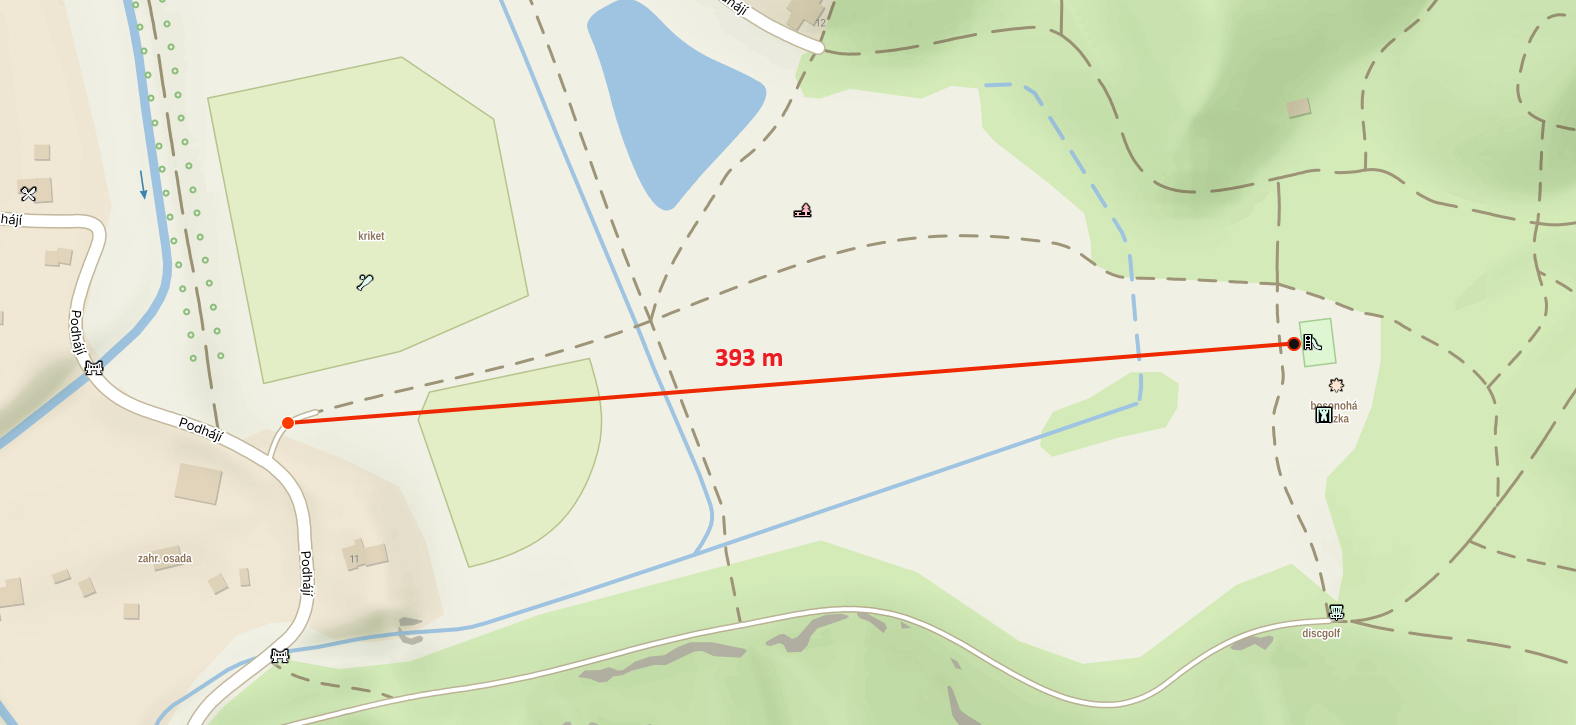
\includegraphics[width=0.8\textwidth]{text/PraktickaCast/img/mapa-zamilec-semafor.png}
  \caption{Mapa zobrazující polohu komunikujících zařízení \cite{MereniDosahuSemaforu-zamilec}}
  \label{Semisemafor-dosah-zamilec}
\end{figure}

Při testování v~lese se~dosah výrazně zkrátí, především pokud v~cestě signálu stojí např. hustý keř.
Přesto jsem ale vetšinou neměl problém navázat spojení na~vzdálenosti do~padesáti metrů.
